\section{Introduction}

As discussed in the first chapter, a transcriptional regulatory module is a set of genes that is regulated by a common set of \acp{TF}. A considerable amount of work has been carried out to determine the network of inter-relationships between these regulatory modules, with the aim of understanding how they act together in order to carry out the complex biological functions of a cell. Microarrays allow us to study a large proportion of genome expression simultaneously. These expression data have been used to build models of the regulatory networks. In some of the recent work, \textit{integrative genomics}, in which data from experiments relating to different conditions or even different organisms are merged together, has been suggested as a method to discover these regulatory modules \citep{amos05integrative,segal04module}. The approach compensates for the fact that the models have a very large number of variables (genes) whereas the number of repeats of microarray experiments is typically quite small. Thus, for a typical single experiment, there is not enough data to model the regulatory modules reliably. Another justification for the integrative approach is that, in evolution, many genes are believed to have similar roles in different organisms and so collective analysis should help to counter experimental error in individual experiments.  

The motivation behind the research presented in this chapter is that, in our view, \textit{blind} integrative genomics can lead to misleading or incorrect results. Researchers conduct experiments with clear objectives in mind. For example, research conducted on yeast to study meiosis will profile gene expression in sporulation media and will have clear meiotic signal in the data. But, hardly any of these conditions will be in common with the experiments related to stress conditions on yeast. Integration should be used when we are \textit{only} concerned about either the background patterns or the most dominant patterns, and are not interested in patterns that may be visible in certain individual experiments. The global regulatory module network is the sum of smaller local regulatory module networks and by taking the integrative approach we run the risk that significant information from individual networks will be masked by the pooling process.

We believe that integrative genomics can sometimes be a useful technique. Our hypothesis is that as microarrays from different experimental conditions but same experiment type, for example stress, are merged, we should be able to readily identify stress specific regulatory modules. The clusters of co-regulated genes obtained should reinforce the local (stress specific) regulatory modules while suppressing the noise. By contrast, when microarrays from various different experiment types are merged together then the local (dataset specific) regulatory modules would be masked by conflicting patterns from other diverse datasets. Only sets of the genes that are strongly expressed among the majority of the conditions for which datasets have been mixed would be observed to behave in a consistent manner while the other genes would be expressed in an unpredictable manner. This should result in regulatory modules that are not very similar to the modules obtained with the original datasets.

One possible way of determining the similarity between datasets is using a statistical measure like the Kullback-Leibler divergence between the distribution of the different datasets \citep{ernstwit2004statis_microarrays}. We computed the difference in data distributions of various distinct and progressively mixed microarray datasets as discussed later. However, the problem with Kullback-Leibler divergence or other statistical methods is that such a theoretical measure is not guaranteed to be a good indicator of \textit{functional} similarity. They don't say much about how the final clusters are affected when we mix datasets. Therefore we validated our results by taking the functional route and studying the eventual effects directly by calculating the similarity among the resulting modules. We carried out experiments in which we obtained regulatory modules from various datasets and their mixtures and then measure their similarities to each other. In this way, we show that progressive mixing of data of differing types inhibits the discovery of local regulatory modules at the cost of more dominant regulatory modules. 

For our experiments, we chose to use the Module Networks algorithm \citep{segal03module} (refer Chapter-2), which is a well established approach and has had recognised success in finding biologically relevant modules. For measuring the similarities among the regulatory gene modules resulting from this algorithm, we chose to use the \textit{modified Rand Index} \citep{hubert85comparing} which has been shown to be a very stable measure of partition similarity. To our knowledge, there hasn't been any thorough study investigating the effects of mixing diverse datasets on the resulting clusters. We also haven't seen any research on understanding the correlation between theoretical data distributions and its impact on the resulting clusters.

\section{Methodology}\label{method}
In order to validate our hypothesis, we chose to work with two very diverse datasets compiled from yeast experiments. One of them is from experiments to study the gene expression when yeast is exposed to stress conditions. The other dataset was from the study of cell-cycle related genes in which the pattern of activity is very different from the previous one. The expression of genes when stress conditions are created is much more drastic (both repressed and induced genes) than the normal cell-cycle, where optimal conditions are created for growth and the expression levels are much smaller. We want to show how progressive dilution of these two datasets with other dissimilar datasets affects the similarity among resulting clusters. We would expect that, as we dilute the datasets, the resulting cluster similarity to the original dataset cluster decreases.

All the data used in our analysis were taken from the \ac{SMD} \citep{sherlock01smd} which hosts c-DNA microarray data-sets from various experimenters. We decided to focus our study on yeast as the regulatory mechanisms in more complex organisms are more involved and yeast has been studied extensively in recent years. We started with analysing data by individual researchers for experiments related to stress. In particular, we used data from \citet{gasch00genomicexpn} submitted by A.P. Gasch which we refer to as DS-STRESS1 (76 microarrays), \citet {saldanha04nutritional} called DS-STRESS2 (49 microarrays) and \citet{gasch00genomicexpn} submitted by P. Spellman called DS-STRESS3 (41 microarrays). We merged all 183 stress related microarray slides available (not only the above three) to create the data set that we refer to as DS-STRESS. To compare these clustering against an entirely different category, we took 93 microarray data sets for cell-cycle experiments \citep{spellman98comprehensive} referred to as DS-CCYCLE. A further mixing of both stress and cell-cycle data created a data set that was named DS-STRESS-CCYCLE (276 microarrays). Finally, we pooled all the available data (523 microarrays) for yeast (not only stress and cell-cycle) and named it DS-ALL. The clusters resulting from all these different data groupings were compared. In order to have a reference point to compare the similarity values, we also generated a random microarray dataset for all the genes by sampling random numbers from a Gaussian distribution with zero mean and unit standard deviation. This dataset was named DS-RANDOM.

To analyze the data we did some standard pre-processing to the datasets. We used the $log_{2}$ of the ratio of the mean of Channel 2 (experimental expression) to the mean of Channel 1 (control expression). We also used total intensity normalization which is based on the assumption that the average log ratio on the array should be zero. Having organised the data, we did three types of studies with the following further processing.

\begin{enumerate}
\item We took all the data described above without further processing.

\item We filtered the genes by choosing those where log(base2) ratio had changed by two fold at least once among all experiments. This retains only those genes that have shown significant change in their expression.

\item We scale normalized each of the above data-sets (without any filtering) across slides to account for different experimental conditions or different data-sets by using a variant of \ac{MAD} \citep{yang02normalization}. Note that this is different from normalizing microarray replicates for removing noise. The data that we are using has already been normalized to account for that. \ac{MAD} is a measure of statistical dispersion and is a more robust estimator of scale than the sample variance or standard deviation. MAD is unaffected by the magnitude of the distances of a small number of outliers whereas in the standard deviation, the distances from the mean are squared, therefore, large deviations are weighted more heavily, and thus outliers can heavily influence it. For our computations, the \ac{MAD} for the $i_{th}$ slide (or condition) is given by
\begin{equation}
MAD_{i}=median_{j}\{\mid M_{ij}-median_{j}(M_{ij}) \mid\}
\end{equation} 
where $j$ ranges across all the genes, $i$ ranges across all the slides (conditions) and $M_{ij}$ is the individual microarray value. We compute the \ac{MAD} value for all the slides and then normalize this score for each slide by taking into account other slides.
\begin{eqnarray}
{a}_{i}&=&\frac{MAD_{i}}{\sqrt[I]{\Pi_{i=1}^{I}MAD_{i}}} \\
M_{ij}(final) &=& \frac{M_{ij}}{a_{i}^{2}} 
\end{eqnarray}

As suggested by the authors, we have divided each value for slide $i$ by $a_{i}^{2}$. This normalization takes into account the \acp{MAD} for all slides and has been found as a reliable way to normalize variation across slides in microarray studies \citep{yang02normalization}.

\end{enumerate}

\subsection{Kullback Leibler divergence among datasets}\label{kl-divergence}
Before we start computing the cluster similarity among datasets, we first need to understand how different (quantitatively) the underlying data distributions are. For this, we have used the \ac{KL} divergence which is a statistical measure to compare distributions. 

For two distributions F and G with densities f and g respectively, the \ac{KL} divergence between them is defined as 
\begin{equation}
d_{KL}(F,G) = \int_{-\infty}^{\infty}f(x)log\frac{f(x)}{g(x)}dx
\end{equation}

However, \ac{KL} divergence is not a distance measure as it lacks symmetry (($d_{KL}(F,G)\neq d_{KL}(G,F)$)), i.e., the \ac{KL} divergence from F to G is not the same as from G to F. There have been some suggestions regarding how to make it symmetric. \citet{Jeffreys46} suggest that it should be modified to 

\begin{equation}
d_{Jeffreys}(F,G) = \frac{d_{KL}(F,G) + d_{KL}(G,F)}{2} \label{KL-Jeffreys}
\end{equation}
which is the mean of both the values. \citet{Johnson01symmetrizing} suggest the harmonic mean and name it as resistor-average mean
\begin{equation}
\frac{1}{d_{Resistor}(F,G)} = \frac{1}{d_{KL}(F,G)} + \frac{1}{d_{KL}(G,F)} 
\end{equation}

We have used the $d_{Jeffreys}$ to validate our results. Determining the underlying distribution of microarray data is another challenge, and more so with so few replicates. We have assumed that the gene expression data across slides (experiments or conditions) has a Gaussian distribution following \citet{ernstwit2004statis_microarrays} who have found that after a logarithmic transformation, most microarray gene expression values across slides have a Gaussian distribution. Another key benefit is that a Gaussian distribution yields an analytically simple and elegant computable form. If $r_{F}$ and $r_{G}$ replicate arrays are spotted for conditions F and G and p is the total number of genes then the two microarray datasets (F and G) could be represented as
\begin{eqnarray*}
f_{ij}: i = 1,\dots p, j = 1,\dots ,r_{F} \\
g_{ij}: i = 1,\dots p, j = 1,\dots ,r_{G}
\end{eqnarray*} 

and the empirical \ac{KL} divergence under the assumption of normality (Gaussian distribution) can be calculated as \citep{ernstwit2004statis_microarrays}

\[
\hat{d}_{KL}(F,G) = \sum_{i=1}^{p} \big[ log \frac{\hat{\sigma}_{gi}}{\hat{\sigma}_{fi}} + \frac{1}{2} \big( \frac{\hat{\sigma}_{fi}^2}{\hat{\sigma}_{gi}^2} + \frac{(\hat{\mu}_{gi}-\hat{\mu}_{fi})^2}{\hat{\sigma}_{gi}^2} -1 \big) \big]
\]
 
where 
\begin{eqnarray}
\hat{\mu}_{fi} &=& \frac{1}{r_{F}}\sum_{j=1}^{r_{F}}f_{ij} \\
\hat{\sigma}_{fi} &=& \frac{1}{r_{F}-1}\sum_{j=1}^{r_{F}}(f_{ij}-\hat{\mu}_{fi})^2
\end{eqnarray}
are the sample mean and variance of the observations associated with the $i_{th}$ gene. It should be noted that this assumes that each of the genes have a univariate Gaussian distribution and they are independent of each other. In essence we are computing pairwise \ac{KL} divergence between corresponding gene replicate data from two different experiments.

\subsection{Cluster similarity}\label{cluster_similarity}
For clustering, we have used the software package Genomica \citep{segal03module} which has been provided by the authors of the Module Network algorithm. The reason we chose this algorithm was because it has been shown in literature to identify biologically meaningful clusters. Its clustering process is driven by the expression of known TFs. The algorithm works as follows: given a gene expression dataset and a precompiled set of candidate regulatory genes, it simultaneously searches for a partition of genes into modules, and for a regulation program for each module that explains the behaviour of the genes in the module. It uses an \ac{EM} approach to do the search. For each module, the procedure searches for a regulation program that provides the best prediction of expression profiles of the genes in the module as a function of the expression of a subset of genes from the candidate regulator set. The approach is iterative and runs till convergence, refining both the regulation program and the gene modules in each iteration. 

This algorithm, apart from microarray data, also requires a list of \acp{TF} as prior knowledge on which to base the clustering. Our TFs were taken from the Yeastract database \citep{Teixeira06yeastract}\footnote{using their web interface \url{http://yeastract.com/} in Sept. 2006 when it had 145 TFs}. 

Since we are comparing the results on different data-sets our goal is to check the closeness of these resulting clusters (on different data-sets). This closeness was validated using \textit{cluster similarity} as described in the next section.

\subsection{Cluster similarity indices}
In order to compare the clusterings obtained on the different datasets, we need a measure of similarity. We have chosen a well established measure of clustering similarity - the \textit{adjusted Rand's Index} - which was proposed by \citet{hubert85comparing}. 

The Rand's index works on the concept of pair-wise matching on each of the cluster sets that are being compared. Given a set of objects of cardinality $n$, $S = {s_1, . . . , s_n}$, suppose we obtain two clusterings $C1$ and $C2$ such that $C1 = {c1_1, . . . , c1_k}$ and $C2 = {c2_1, . . . , c2_k }$ where $\bigcup_{i=1}^{k}c1_{i} = S = \bigcup_{j=1}^{k}c2_{j}$. If:
\begin{eqnarray*}
N_{11} & = & \mbox{number of pairs of objects in the same cluster in both C1 and C2}\nonumber\\
N_{00} & = & \mbox{number of pairs of objects in different clusters in both C1 and C2}\nonumber\\
N_{01} & = & \mbox{number of pairs of objects in different clusters in C1 but same cluster in C2}\nonumber\\
N_{10} & = & \mbox{number of pairs of objects in the same cluster in C1 but different clusters in C2}\nonumber\\
\end{eqnarray*}

then \textit{agreement(A)} is the sum of $N_{11}$ and $N_{00}$ and \textit{disagreement(D)} is the sum of $N_{01}$ and $N_{10}$. \textit{A} is the sum of pairs where both clusterings agree and \textit{D}, where both disagree. The Rand's index is simply the fraction in \textit{agreement} to the total (\textit{agreement} + \textit{disagreement}), i.e.,
\[
R_{C1C2}=\frac{(N_{11} + N_{00})}{(N_{11} + N_{00}+N_{01} + N_{10})}
\]
and its value lies between 0 and 1. When the two partitions are identical, the Rand's index is 1. It falls to 0 when the two clusters have nothing in common. The biggest drawback of this index is that it doesn't have a good spread of values. Another problem with the Rand's index is that the \textit{expected} value of two random partitions does not take a constant value. This is an expected statistical property of any good index to compare clusterings. The modified version of the Rand's index - also known as \textit{adjusted} or \textit{modified Rand's index} corrects for this by assuming the general form
\[
R_{C1C2adj}=\frac{\text{index value - expected(index value)}}{\text{maximum(index value) - expected(index value)}}
\]
For a detailed derivation of the analytical form of this equation, please refer \citet{hubert85comparing}. 
\begin{table}[t]
\centering
\begin{tabular}{|c|c|c|}
\hline
Datasets & \multicolumn{2}{|c|}{Cluster Similarity Index} \\
& Rand's &  \textit{adjusted} Rand's \\
\hline
DS-STRESS3 \& DS-RANDOM & 0.945 & 0.001 \\
DS-STRESS3 \& DS-CCYCLE & 0.946 & 0.100 \\ 
DS-STRESS3 \& DS-STRESS3 (different runs) & 0.957 & 0.453 \\
\hline 
\end{tabular}
\caption[Comparison of Rand's Index and \textit{adjusted} Rand's Index]{Comparison of Rand's Index and \textit{adjusted} Rand's Index. Spread of values by Rand's index is skewed while the \textit{adjusted} Rand's index shows a very wide spread of values.}
\label{tab:rand_vs_adjustedrands}
\end{table}

Its maximum value is 1 and its expected value in the case of random clusters is 0. Based on an extensive empirical comparison of several such measures, \citet{milligan85exam} recommended this index as the best measure of agreement even when comparing partitions having different numbers of clusters. 
We did a comparison of Rand's and \textit{adjusted} Rand's index on our clustering results. Table-\ref{tab:rand_vs_adjustedrands} shows that the spread of values by Rand's index is skewed (all the values seem to be above 0.94). On the other hand, the \textit{adjusted} Rand's index shows a very wide spread of values. Based on this justification, we chose to use it for all our cluster comparisons. Our whole methodology is summarised in Algorithm-\ref{alg:cluster_comparison}.

\begin{algorithm}
\caption{Summary of methodology}
\label{alg:cluster_comparison}
\begin{algorithmic}[1]

\STATE Pre-process the datasets using the filtering and normalization steps discussed earlier to create 3 separate datasets (normal, filtered and scale normalized).
\STATE Process (mix) datasets so that they contain data from progressively diverse microarray experiments. 
\STATE Run clustering algorithm over each of these resulting datasets. 
\STATE Calculate cluster similarity among the resulting sets of clusters.
\STATE Compute \ac{KL} divergence among all these datasets.
\STATE Compute the correlation coefficient between the cluster similarities and \ac{KL} divergences.
\end{algorithmic}
\end{algorithm}

\section{Results}
\subsection{Cluster similarity among datasets}
\begin{sidewaystable}[htp]
\begin{center}

\subtable[Cluster variation among stress datasets]
{
\label{results:unnorm:intra_class_clustering_variation}
\begin{tabular}{|c|c|c|c|}
\hline
& DS-STRESS1 & DS-STRESS2 & DS-STRESS3 \\

\hline

DS-STRESS1 & 0.5420 (0.0161) & 0.0261 (0.0024) & 0.0709 (0.0024)\\ \hline
DS-STRESS2 & -      & 0.5070 (0.0162) & 0.0213 (0.0014)\\ \hline
DS-STRESS3 & -      & -      & 0.5227 (0.0483)\\ \hline

\end{tabular}
}

\subtable[Comparison of clustering of individual stress datasets versus progressively mixed datasets]
{
\label{results:unnorm:stress_vs_mixed}
\begin{tabular}{|c|c|c|c|c|c|}
\hline
 & DS-STRESS & DS-STRESS-CCYCLE & DS-ALL & DS-CCYCLE & DS-RANDOM\\
\hline
DS-STRESS1 & 0.1616 & 0.1368 & 0.1186 & 0.0354 & 0.0003 \\ \hline
DS-STRESS2 & 0.0606 & 0.0555 & 0.0528 & 0.0176 & 0.0001 \\ \hline
DS-STRESS3 & 0.1105 & 0.1109 & 0.0989 & 0.0309 & 0.0001 \\ \hline

\end{tabular}
}

\subtable[Comparison of cell-cycle and stress to mixed data clustering]
{
\label{results:unnorm:cell-cycle_vs_mixed}
\begin{tabular}{|c|c|c|c|c|c|}
\hline
 & DS-STRESS & DS-CCYCLE & DS-STRESS-CCYCLE & DS-ALL & DS-RANDOM \\ \hline
DS-CCYCLE & 0.0418 & 0.4736 & 0.0783 & 0.0638 & 0.0007 \\ \hline
DS-STRESS & 0.5288 & 0.0418 & 0.2197 & 0.1784 & 0.0003 \\ \hline
\end{tabular}
}
\caption{Cluster similarity among full (non scale-normalized) datasets}
\label{results:unnorm}

\end{center}
\end{sidewaystable}

\begin{sidewaystable}[htp]
\begin{center}

\subtable[Cluster variation among stress datasets]
{
\label{results:filtered:intra_class_clustering_variation}
\begin{tabular}{|c|c|c|c|}
\hline
& DS-STRESS1 & DS-STRESS2 & DS-STRESS3 \\
\hline

DS-STRESS1 & 0.6600 & 0.1747 & 0.2417 \\ \hline
DS-STRESS2 & -      & 0.5500 & 0.1155 \\ \hline
DS-STRESS3 & -      & -      & 0.5933 \\ \hline

\end{tabular}
}

\subtable[Comparison of clustering of individual stress datasets versus progressively mixed datasets]
{
\label{results:filtered:stress_vs_mixed}
\begin{tabular}{|c|c|c|c|c|c|}
\hline
 & DS-STRESS & DS-STRESS-CCYCLE & DS-ALL & DS-CCYCLE & DS-RANDOM\\
\hline
DS-STRESS1 & 0.3425 & 0.3378 & 0.3434 & 0.0981 & 0.0037 \\ \hline
DS-STRESS2 & 0.1060 & 0.0920 & 0.0759 & 0.0252 & 0.0022 \\ \hline
DS-STRESS3 & 0.2470 & 0.2534 & 0.2325 & 0.0925 & 0.0023 \\ \hline
\end{tabular}
}

\subtable[Comparison of cell-cycle and stress to mixed data clustering]
{
\label{results:filtered:cell-cycle_vs_mixed}
\begin{tabular}{|c|c|c|c|c|c|}
\hline
 & DS-STRESS & DS-CCYCLE & DS-STRESS-CCYCLE & DS-ALL & DS-RANDOM \\ \hline
DS-CCYCLE & 0.0663 & 0.4768 & 0.0812 & 0.0614 & 0.00068 \\ \hline
DS-STRESS & 0.5986 & 0.0663 & 0.3067 & 0.2244 & 0.0013 \\ \hline
\end{tabular}
}
\caption{Cluster similarity among filtered (non scale-normalized) datasets}
\label{results:filtered}

\end{center}
\end{sidewaystable}

\begin{sidewaystable}[htp]
\begin{center}

\subtable[Cluster variation among stress datasets]
{
\label{results:norm:intra_class_clustering_variation}
\begin{tabular}{|c|c|c|c|}
\hline
& DS-STRESS1 & DS-STRESS2 & DS-STRESS3 \\
\hline
DS-STRESS1 & 0.4446 & 0.0125 & 0.0340 \\ \hline
DS-STRESS2 & -      & 0.4740 & 0.0086 \\ \hline
DS-STRESS3 & -      & -      & 0.4652 \\ \hline
\end{tabular}
}

\subtable[Comparison of clustering of individual stress datasets versus progressively mixed datasets]
{
\label{results:norm:stress_vs_mixed}
\begin{tabular}{|c|c|c|c|c|c|}
\hline
 & DS-STRESS & DS-STRESS-CCYCLE & DS-ALL & DS-CCYCLE & DS-RANDOM\\
\hline
DS-STRESS1 & 0.0550 & 0.0468 & 0.0532 & 0.0070 & 0.0001 \\ \hline
DS-STRESS2 & 0.0186 & 0.0165 & 0.0192 & 0.0025 & 0.0003 \\ \hline
DS-STRESS3 & 0.0419 & 0.0345 & 0.0364 & 0.0053 & 0.0004 \\ \hline
\end{tabular}
}
\subtable[Comparison of cell-cycle and stress to mixed data clustering]
{
\label{results:norm:cell-cycle_vs_mixed}
\begin{tabular}{|c|c|c|c|c|c|}
\hline
 & DS-STRESS & DS-CCYCLE & DS-STRESS-CCYCLE & DS-ALL & DS-RANDOM \\ \hline
DS-CCYCLE & 0.0068 & 0.5310 & 0.0117 & 0.0093 & 0.0008 \\ \hline
DS-STRESS & 0.4751 & 0.0068 & 0.0781 & 0.0623 & 0.0003 \\ \hline
\end{tabular}
}
\caption{Cluster similarity among full (scale-normalized) datasets}
\label{results:norm}
\end{center}
\end{sidewaystable}


The results of cluster similarity computations are in Tables-\ref{results:unnorm}, \ref{results:filtered}, and \ref{results:norm}. The clustering algorithm groups together \textit{functionally} similar genes. By using the modified Rand index, we measure the similarity among the resulting sets of clusters. We ran the clustering algorithm 4 times for each dataset and have reported the mean values of all these runs. This was done because the initialization of the clustering algorithm is done by another non-deterministic algorithm. We observed that the final results did not have significant standard deviation (values in brackets in Table-\ref{results:unnorm}\subref{results:unnorm:intra_class_clustering_variation}). For clarity of presentation, we have not reported standard deviation values in remaining tables.

We first compared the individual stress datasets to each other to compare how similar the various runs of the same dataset are as well as to other stress datasets. We then compared each of the stress datasets against DS-STRESS, DS-STRESS-CCYCLE, DS-ALL, DS-CCYCLE which are increasingly distant from the stress datasets as described earlier. As a reference, we also compared them against DS-RANDOM which is a randomly generated dataset and gives us a baseline against which to compare the rest of the similarity values. 

The values in Table-\ref{results:unnorm}\subref{results:unnorm:intra_class_clustering_variation}, \ref{results:filtered}\subref{results:filtered:intra_class_clustering_variation}, and \ref{results:norm}\subref{results:norm:intra_class_clustering_variation} indicate the level of similarity among the same type of datasets. The results in all three suggest that even among datasets of the same type, e.g. stress, there is considerable variation in similarity values, for example DS-STRESS1 and DS-STRESS3 are much more similar to each other than to DS-STRESS2 which could be explained from the fact that they were done under similar conditions. We also observe that DS-STRESS1 is slightly more similar to DS-STRESS2 than DS-STRESS3 across all three classes. Another interesting observation is that DS-STRESS1 is more similar to DS-CCYCLE than DS-STRESS2 pointing to the fact that there could be large variations in results even under similar conditions.

Results in Table-\ref{results:unnorm}\subref{results:unnorm:stress_vs_mixed} show the expected trend. As diverse datasets are merged, the similarity of the resulting clusters to the original dataset falls progressively. We observe that all three stress datasets are most similar to the combined stress dataset (DS-STRESS). As the combined stress data is mixed with cell-cycle data, the similarity value falls. Since DS-ALL is even more diluted in stress data (it combines even more non-stress data), the similarity value has fallen further. All the stress datasets' similarity to DS-CCYCLE is very low, as we expected because of very different nature of expression in these diverse experiments. The similarity values for the random data-set are near zero in all the cases. Another interesting observation is that stress dataset seem to be very dominant in the final mixture (DS-ALL) as we see that the similarity values haven't fallen a lot between DS-STRESS and DS-ALL. Across all three stress datasets, we observe that the similarity values across DS-STRESS, DS-STRESS-CCYCLE and DS-ALL are much closer than the rest.

Table-\ref{results:unnorm}\subref{results:unnorm:cell-cycle_vs_mixed} shows the results at a more macro level using all stress data and all cell-cycle data. These results generalise and substantiate our earlier observations as the same trends are more robust here because of aggregation of data. Again we observe that similarity values across DS-STRESS, DS-STRESS-CCYCLE and DS-ALL are much closer than the rest.

When we filtered the datasets, retaining only those genes that changed their expression value by two fold at least once, the results, shown in Table-\ref{results:filtered} are somewhat different from the previous study. We observe that the similarity values are much higher when compared to the earlier unnormalized datasets. An explanation for this is that as we have retained only genes that are highly expressed, the total number of genes is smaller, and the uncorrelated background expression has been reduced. Results in Table-\ref{results:filtered}\subref{results:filtered:intra_class_clustering_variation} show similar trend as the earlier one where DS-STRESS1 and DS-STRESS3 are much more similar to each other than to DS-STRESS2. DS-STRESS1 is also slightly more similar to DS-STRESS2 than DS-STRESS3. Like the previous study, the similarity values in Table-\ref{results:filtered}\subref{results:filtered:stress_vs_mixed} indicate that DS-STRESS, DS-STRESS-CCYCLE and DS-ALL are quite similar to each other. The similarity values are in similar range and sometimes the trend is not very sharply delineated among them. 

A further look at Table-\ref{results:filtered}\subref{results:filtered:cell-cycle_vs_mixed} indicates that the cell-cycle data is almost equally dissimilar from each of the mixes (DS-STRESS, DS-STRESS-CCYCLE, and DS-ALL) like the previous study. This indicates that the stress data is somehow dominating other data in the combined datasets. The combined stress data is showing the expected trend as its similarity values are falling as more diverse data is mixed.

Our third study used scale normalization (with MAD) in order to bring all the expression values across various different experimental conditions into the same range. We chose to do this after observing that the stress expression values fall in a much larger range than the cell cycle values, which might explain the disparate similarity values found when the datasets were merged together in the previous two studies. After scale normalization, we got some interesting results as shown in Table-\ref{results:norm}. The similarity values fell considerably, especially among different types of datasets. We believe that the reason for this is that as the range of expression values have been brought to a similar scale, the clustering algorithm is not able to identify dominant clusters as clearly as earlier. 

Table-\ref{results:norm}\subref{results:norm:intra_class_clustering_variation} show similar trend as the earlier one where DS-STRESS1 and DS-STRESS3 are much more similar to each other than to DS-STRESS2. DS-STRESS1 is again slightly more similar to DS-STRESS2 than DS-STRESS3. Based on the results so far, it is possible that the DS-STRESS2 is not representative of the combined stress behaviour indicating that the data may be of lower quality. 

Table-\ref{results:norm}\subref{results:norm:stress_vs_mixed} shows that DS-STRESS, DS-STRESS-CCYCLE and DS-ALL are again quite similar to each other as the similarity values are in similar range and sometimes the trend is not very sharply delineated among them. Table-\ref{results:norm}\subref{results:norm:cell-cycle_vs_mixed} shows similar trends as seen previously.

\subsection{KL divergence among datasets}
\begin{table}[p]\tiny
\begin{center}

\subtable[KL Divergence among stress datasets]
{
\begin{tabular}{|c|c|c|c|}
\hline
& DS-STRESS1 & DS-STRESS2 & DS-STRESS3 \\

\hline

DS-STRESS1 & 0	& 4843.3 & 1329.0 \\ \hline
DS-STRESS2 & -	& 0 & 4712.3 \\ \hline
DS-STRESS3 & - & - & 0 \\ \hline

\end{tabular}
\label{results:unnorm:kldiv:intra_class_kldivergence}

}

\subtable[KL Divergence among individual stress datasets versus progressively mixed datasets]
{
\begin{tabular}{|c|c|c|c|c|c|}
\hline
 & DS-STRESS & DS-STRESS-CCYCLE & DS-ALL & DS-CCYCLE \\
\hline
DS-STRESS1 & 1066.2 & 897.29 & 1131.0 & 1885.25\\ \hline
DS-STRESS2 & 1226.6 & 1598.2 & 1646.0 & 5116.5\\ \hline
DS-STRESS3 & 1139.5 & 1039.2 & 1234.1 & 2747.0\\ \hline

\end{tabular}
\label{results:unnorm:kldiv:stress_vs_mixed_kldivergence}
}

\subtable[KL Divergence among cell-cycle, stress and mixed datasets]
{
\begin{tabular}{|c|c|c|c|c|c|}
\hline
 & DS-STRESS & DS-CCYCLE & DS-STRESS-CCYCLE & DS-ALL \\ \hline
DS-CCYCLE & 2186.5 & 0 & 1190.7 & 1805.8 \\ \hline
DS-STRESS & 0 & 2186.5 & 125.5& 194.5 \\ \hline
\end{tabular}
\label{results:unnorm:kldiv:cell-cycle_vs_mixed_kldivergence}
}
\caption{KL Divergence among full (non scale-normalized) datasets}
\label{results:unnorm:kldiv}

\end{center}
\end{table}

%%%%%%%% next table %%%%%%%%%%%%%%%%%%%%%%%%%%%%%%%%%%%%%
%%%%%%%%%%%%%%%%%%%%%%%%%%%%%%%%%%%%%%%%%%%%%%%%%%%%%%%%%
\begin{table}[p]\tiny
\begin{center}

\subtable[KL Divergence among stress datasets]
{
\begin{tabular}{|c|c|c|c|}
\hline
& DS-STRESS1 & DS-STRESS2 & DS-STRESS3 \\

\hline

DS-STRESS1 & 0	& 475.5 & 242.7 \\ \hline
DS-STRESS2 & -	& 0 & 367.9 \\ \hline
DS-STRESS3 & - & - & 0 \\ \hline

\end{tabular}
\label{results:filtered:kldiv:intra_class_kldivergence}

}

\subtable[KL Divergence among individual stress datasets versus progressively mixed datasets]
{
\begin{tabular}{|c|c|c|c|c|c|}
\hline
 & DS-STRESS & DS-STRESS-CCYCLE & DS-ALL & DS-CCYCLE \\
\hline
DS-STRESS1 & 130.60 &         121.20 &         129.30 & 217.50 \\ \hline
DS-STRESS2 & 670.75   &       952.40  &        1011.20 & 638.40 \\ \hline
DS-STRESS3 & 132.10   &       226.65   &       199.20  & 380.70 \\ \hline 
\end{tabular}
\label{results:filtered:kldiv:stress_vs_mixed_kldivergence}
}

\subtable[KL Divergence among cell-cycle, stress and mixed datasets]
{
\begin{tabular}{|c|c|c|c|c|c|}
\hline
 & DS-STRESS & DS-CCYCLE & DS-STRESS-CCYCLE & DS-ALL \\ \hline
DS-CCYCLE & 340.5 & 0.0 &  198.3 & 297.5 \\ \hline
DS-STRESS & 0.0 & 340.5 & 92.0 & 147.7 \\ \hline
\end{tabular}
\label{results:filtered:kldiv:cell-cycle_vs_mixed_kldivergence}
}
\caption{KL Divergence among filtered (non scale-normalized) datasets}
\label{results:filtered:kldiv}

\end{center}
\end{table}

%%%%%%%% next table %%%%%%%%%%%%%%%%%%%%%%%%%%%%%%%%%%%%%
%%%%%%%%%%%%%%%%%%%%%%%%%%%%%%%%%%%%%%%%%%%%%%%%%%%%%%%%%

\begin{table}[p]\tiny
\begin{center}

\subtable[KL Divergence among stress datasets]
{
\begin{tabular}{|c|c|c|c|}
\hline
& DS-STRESS1 & DS-STRESS2 & DS-STRESS3 \\

\hline

DS-STRESS1 & 0	& 4960.7 & 2116.05 \\ \hline
DS-STRESS2 & -	& 0 & 4390.90 \\ \hline
DS-STRESS3 & - & - & 0 \\ \hline

\end{tabular}
\label{results:norm:kldiv:intra_class_kldivergence}

}

\subtable[KL Divergence among individual stress datasets versus progressively mixed datasets]
{
\begin{tabular}{|c|c|c|c|c|c|}
\hline
 & DS-STRESS & DS-STRESS-CCYCLE & DS-ALL & DS-CCYCLE \\
\hline
DS-STRESS1 & 2885.85   &        2451.55 &         3819.50 & 3179.65\\ \hline
DS-STRESS2 & 1179.95   &        1203.85 &         1501.85 & 7768.15 \\ \hline
DS-STRESS3 & 2244.15   &        1944.65 &         2804.85 & 5644.25\\ \hline

\end{tabular}
\label{results:norm:kldiv:stress_vs_mixed_kldivergence}

}

\subtable[KL Divergence among cell-cycle, stress and mixed datasets]
{
\begin{tabular}{|c|c|c|c|c|c|}
\hline
 & DS-STRESS & DS-CCYCLE & DS-STRESS-CCYCLE & DS-ALL \\ \hline
DS-CCYCLE & 6818.35 &   0.00 & 4947.10 & 7625.75 \\ \hline
DS-STRESS & 0.00 & 6818.35 & 376.70 & 466.65 \\ \hline
\end{tabular}
\label{results:norm:kldiv:cell-cycle_vs_mixed_kldivergence}
}
\caption{KL Divergence among full (scale-normalized) datasets}
\label{results:norm:kldiv}

\end{center}
\end{table}























The results for KL divergence computations using Jeffreys' adjustment (refer eqn-\ref{KL-Jeffreys}) among various datasets are shown in Tables-\ref{results:unnorm:kldiv}, \ref{results:filtered:kldiv}, and \ref{results:norm:kldiv}. Table-\ref{results:unnorm:kldiv} shows the KL divergence among the non-scale normalized datasets. Table-\ref{results:filtered:kldiv} has the results for filtered (non-scale normalized) datasets while Table-\ref{results:norm:kldiv} has the results for the scale-normalized datasets. While cluster similarity was used for \textit{functional} difference among datasets, these denote the \textit{theoretical} difference among the datasets by computing the \ac{KL} divergence between the underlying distributions. One thing to note is that these are \textit{distances} while the values in the cluster similarity section were \textit{similarity} values. Therefore, smaller KL-divergence indicates more similarity. 

Like the computations using cluster similarity, we first compared the individual stress datasets to each other to study their similarity.  The values in Table-\ref{results:unnorm:kldiv}\subref{results:unnorm:kldiv:intra_class_kldivergence}, \ref{results:filtered:kldiv}\subref{results:filtered:kldiv:intra_class_kldivergence}, and \ref{results:norm:kldiv}\subref{results:norm:kldiv:intra_class_kldivergence} indicate the level of similarity among the same type of datasets. Like the results of cluster similarity, the results in all three suggest that even among datasets of the same type, e.g. stress, there is considerable variation in similarity values, for example DS-STRESS1 and DS-STRESS3 are much more similar to each other than to DS-STRESS2 which could be explained from the fact that they were done under similar conditions. We also observe that DS-STRESS1 is slightly less similar to DS-STRESS2 than DS-STRESS3 across all three classes. This is in contrast to the observations in cluster similarity where DS-STRESS1 is slightly more similar to DS-STRESS2 than DS-STRESS3. It could be explained by the fact that clustering involves a number of steps that could loose information.

We then compared each of the stress datasets against DS-STRESS, DS-STRESS-CCYCLE, DS-ALL, DS-CCYCLE which are increasingly distant from the stress datasets as described earlier. As seen in Table-\ref{results:unnorm:kldiv}\subref{results:unnorm:kldiv:stress_vs_mixed_kldivergence}, all the stress datasets' similarity to DS-CCYCLE is very low as we expected because of very different nature of expression in these diverse experiments. Again, as diverse datasets are merged, the similarity of the resulting clusters to the original dataset falls progressively. We again observe that this trend is not very distinct among DS-STRESS, DS-STRESS-CCYCLE and DS-ALL. Like previously, we attribute it to the fact that those datasets are quite similar. Table-\ref{results:unnorm:kldiv}\subref{results:unnorm:kldiv:cell-cycle_vs_mixed_kldivergence} shows the results of the tests at a more macro level using all stress data and all cell-cycle data. These results generalise and substantiate our earlier observations as the trends are more robust here because of aggregation of data. This table has another very interesting result. The values for divergence between DS-STRESS and DS-STRESS-CCYCLE and DS-ALL are extremely low (125.5 and 194.5). This means that they are very close from the perspective of their data distribution. This could be the reason why other datasets' similarity to them were in close range and many times overlapping among them.

When we filtered the datasets, retaining only those genes that changed their expression value by two fold at least once, the results, shown in Table-\ref{results:filtered:kldiv} are again (like cluster similarity) different from the unnormalized data as the similarity values are much higher when compared to the unnormalized datasets. Results in Table-\ref{results:filtered:kldiv}\subref{results:filtered:kldiv:intra_class_kldivergence} show similar trends to the earlier one where DS-STRESS1 and DS-STRESS3 are much more similar to each other than to DS-STRESS2. DS-STRESS1 is slightly less similar to DS-STRESS2 than DS-STRESS3. Like the previous study, the similarity values in Table-\ref{results:filtered:kldiv}\subref{results:filtered:kldiv:stress_vs_mixed_kldivergence} do not show a distinct trend. But Table-\ref{results:filtered:kldiv}\subref{results:filtered:kldiv:cell-cycle_vs_mixed_kldivergence} has the expected trend of falling similarity with increasingly diverse data. It also indicates that DS-STRESS, DS-STRESS-CCYCLE and DS-ALL are quite similar to each other. This reinforces the idea that the stress data is somehow dominating other data in the combined datasets.

Our third study used scale normalization (MAD) in order to bring all the expression values across various different experimental conditions into the same range. Like the results of cluster similarity, the similarity values fell considerably, specially among different types of datasets (Table-\ref{results:norm:kldiv}). Again, we believe that the reason for this is that as the range of expression values have been brought to a similar scale, the clustering algorithm is not able to identify dominant clusters as clearly as earlier. Table-\ref{results:norm:kldiv}\subref{results:norm:kldiv:intra_class_kldivergence} show similar trends to the earlier one where DS-STRESS1 and DS-STRESS3 are much more similar to each other than to DS-STRESS2. DS-STRESS3 is again slightly more similar to DS-STRESS2 than DS-STRESS1. Again the trend in Table-\ref{results:norm:kldiv}\subref{results:norm:kldiv:stress_vs_mixed_kldivergence} is not very distinct while  Table-\ref{results:norm:kldiv}\subref{results:norm:kldiv:cell-cycle_vs_mixed_kldivergence} shows expected trend as seen previously.

%%%%%%%%%%%%%%%%%%%%%%%%%%%%%%%%%%%%%%Correlation indices %%%%%%%%
\subsection{Correlation between KL divergence and cluster similarity}

\begin{table}[t]
\centering
\begin{tabular}{|c|c|c|c|}
\hline
& Non-Scale normalized & Filtered & Scale normalized \\
\hline

DS-STRESS1 & -0.726	& -0.834  & -0.812 \\ \hline
DS-STRESS2 & -0.731	& -0.807  & -0.433 \\ \hline
DS-STRESS3 & -0.776     & -0.932  & -0.576 \\ \hline
DS-STRESS  & -0.967     & -0.952  & -0.978 \\ \hline
DS-CCYCLE  & -0.925     & -0.994  & -0.660 \\ \hline
\end{tabular}
\caption[Pearson's Correlation betwen KL divergence and Cluster similarity]{Pearson's Correlation betwen KL divergence and Cluster similarity. There is a very strong correlation
between the results of KL divergence among the datasets and the cluster similarities.}
\label{results:correlation_clustering_kldivergence}
\end {table}

In order to correlate the findings of \ac{KL} divergence computations with the cluster similarities, we computed the Pearson's Correlation among the corresponding KL divergence values and the cluster similarity values. For each of datasets, DS-STRESS1, DS-STRESS2 and DS-STRESS3, all the observations were combined into a single vector of observations. The results of correlation calculations are shown in Table-\ref{results:correlation_clustering_kldivergence}. It is clear from the results, that for all the datasets, there is a very strong correlation among the results of KL divergence among the datasets and the cluster similarities. The negative values only indicate that the correlation is negative which is expected because cluster similarity values are \textit{similarity} while the KL divergence is a \textit{distance}. If we convert both of them to either similarity or distance then the correlation would turn positive with the magnitude remaining the same. For unnormalised and filtered data, the correlation values are high, indicating strong correlation. The interesting pattern here is that as we move from full data to filtered data (both non scale-normalised) there is a slight improvement in the correlation values. This indicates that filtering of unwanted genes that mostly act as noise makes the datasets cleaner. On the other hand, after normalization, the values are not so strong. As we saw earlier in Table-\ref{results:norm}, even the similarity values had fallen after normalisation. This is the reason why the correlation is not strong here consistently.

Based on the correlation results shown in Table-\ref{results:correlation_clustering_kldivergence}, we consider cluster similarity to be an excellent indicator of dataset similarity. The cluster similarity values are in the range of 0 to 1 and we would like to propose cluster similarity as an index of microarray dataset similarity. It is easy to compute, unlike KL divergence. This index would be especially helpful for researchers who are anyways doing clustering as part of their analysis. This extra step would help them understand if various datasets that they are working on are compatible or not.

\subsection{Effect of data heterogeneity}

\begin{figure}[p]\centering
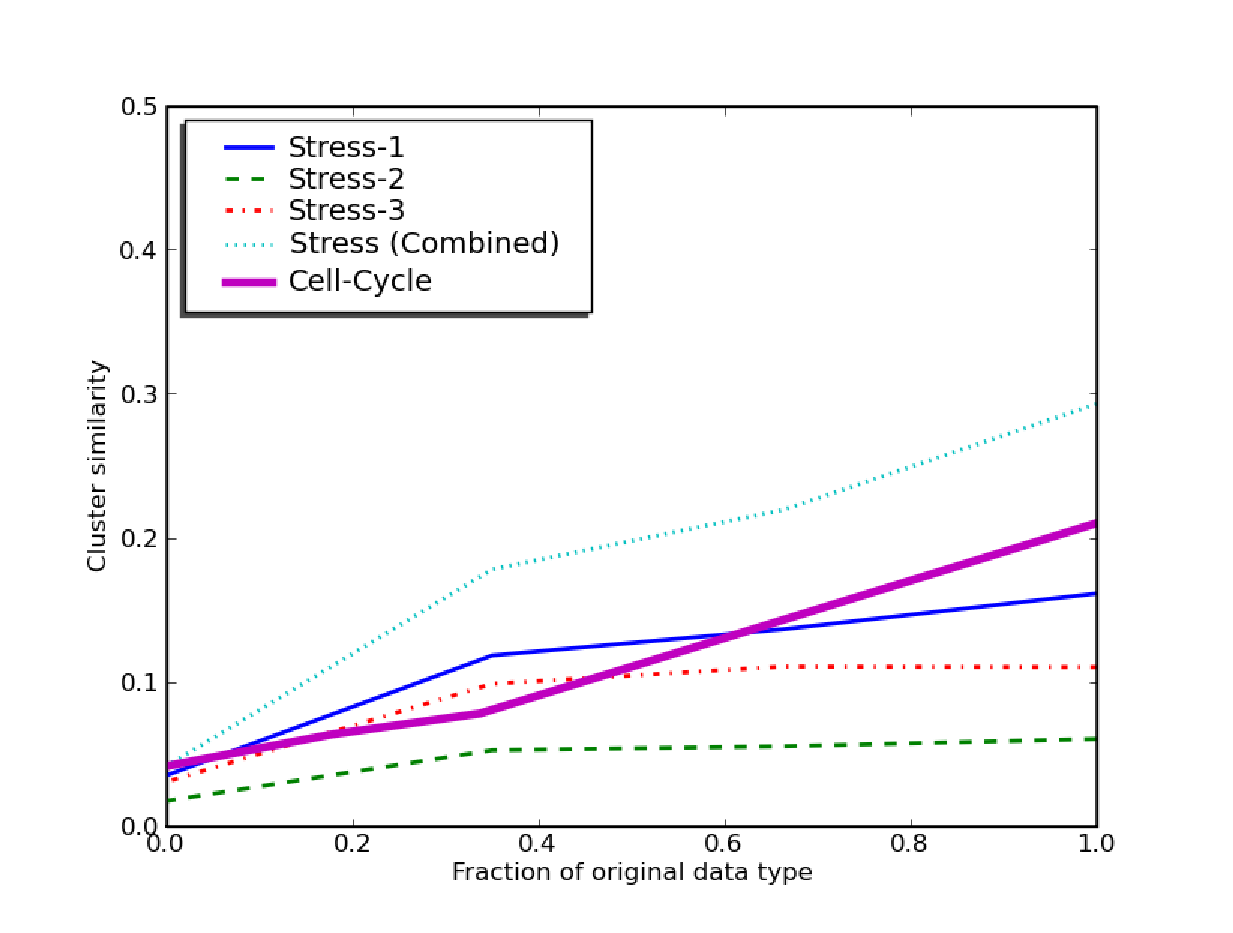
\includegraphics[scale=0.35]{chapter1/plot_unnorm.eps}
\caption{Full (non scale-normalized) data: Variation of cluster similarity with data homogeneity}
\label{graphs:all:unnorm}
\end{figure}

\begin{figure}[p]\centering
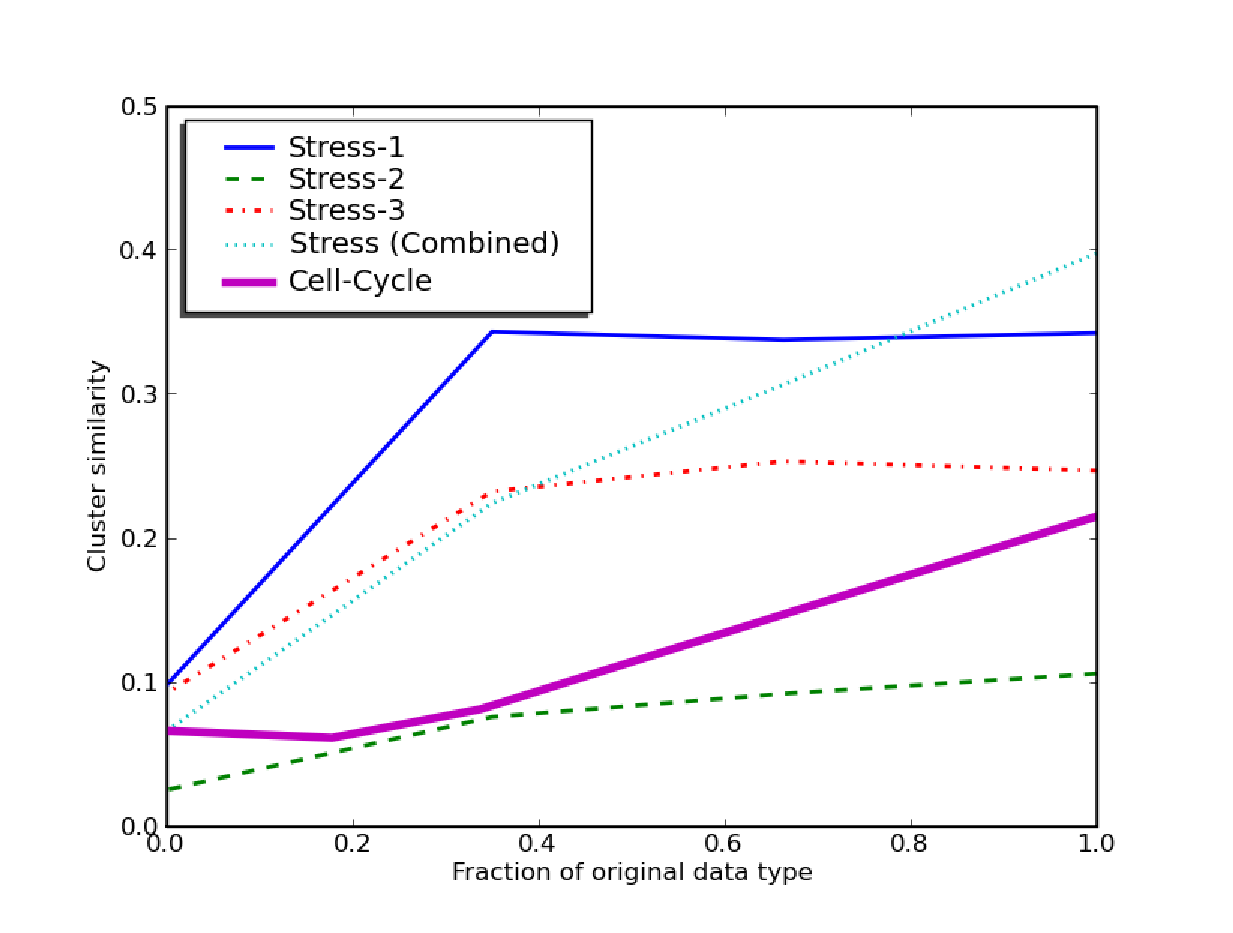
\includegraphics[scale=0.35]{chapter1/plot_filtered.eps}
\caption{Filtered (non scale-normalized) data: Variation of cluster similarity with data homogeneity}
\label{graphs:all:filtered}
\end{figure}

\begin{figure}[p]\centering
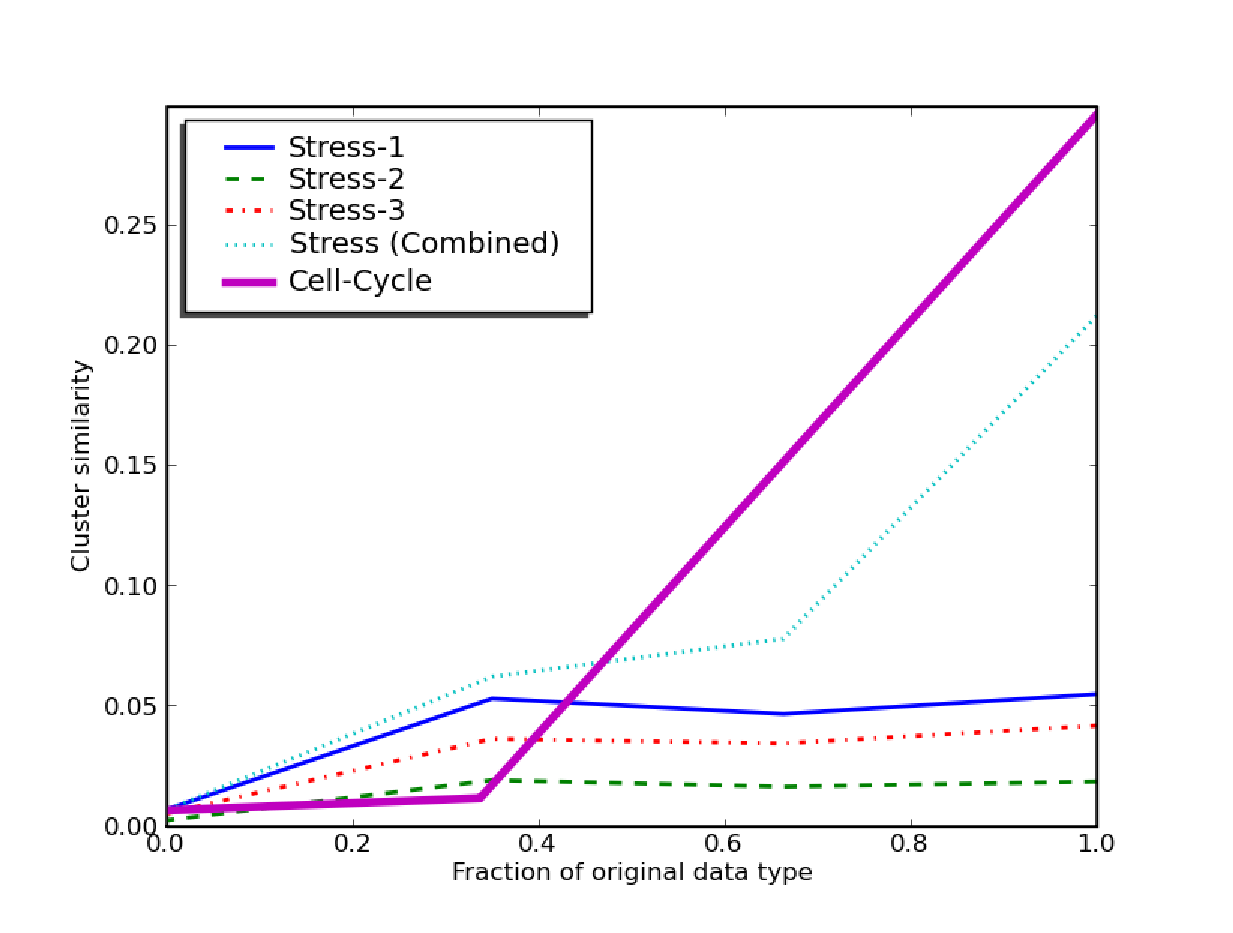
\includegraphics[scale=0.35]{chapter1/plot_norm.eps}
\caption{Full (scale normalized data): Variation of cluster similarity with data homogeneity}
\label{graphs:all:norm}
\end{figure}

We also studied the variation of cluster similarity with the percentage of similar data as shown in Figures - (\ref{graphs:all:unnorm}, \ref{graphs:all:filtered} and \ref{graphs:all:norm}). For each mixed dataset, we calculated the fraction of original data type (e.g stress or cell-cycle) in the resulting mix. Similarity values were then plotted against these fractions. In all the figures, we see the general trend that as the fraction of the original datatype is increasing the cluster similarity values rises. We also observe that the combined datasets (both stress and cell-cycle) show a more consistent upward trend as compared to individual stress datasets. This is consistent with the observations we had in the earlier section and could be attributed to the dominance of stress data when mixed with other types. Figure-\ref{graphs:all:filtered} 
shows a gradually increasing trend though it's not as smooth as Figure-\ref{graphs:all:unnorm} because of the increased dominance of the stress datasets when data is filtered. As seen from Figure-\ref{graphs:all:norm}, the general trend remains that similarity values increase with increasing fraction of similar data. These figures validate our hypothesis that we should be cautious towards integrating diverse datasets as they might be contributing to more noise and removing the original signals from the datasets. When we need to integrate different datasets, we should first compute their similarities and then only integrate similar ones while removing widely diverse ones.
\section{Discussion}
Learning the structure of genetic regulatory module networks has attracted a lot of attention in the past years. We saw a review of these techniques in Chapter-2. Recently, many researchers have focused on integrated approaches where they analyze a big compendium of microarrays gathered from various sources. \citet{hughes00functional} created a reference database or \textit{compendium} of whole-genome microarray data for yeast from 300 diverse mutations and chemical treatments under similar growth conditions. They used this to identify the pathways perturbed by an uncharacterized mutation by computing the similarity of expression of the uncharacterized mutation to the ones in the compendium. 

A similar compendium approach was followed by \citet{amos05integrative} who used data encompassing 1767 conditions from 60 different publications to find regulatory programs. The key difference from \citet{hughes00functional} is that while \citet{hughes00functional} had created the compendium from experiments under similar conditions in a single lab, \citet{amos05integrative} have used data from widely varying conditions. They followed the normalization methods suggested by individual authors to process the individual datasets. However, they did not do any combined (across all conditions) normalization to account for diversity across different datasets. This compendium was then used as a reference against which new data was compared. They used the SAMBA algorithm (refer Chapter-2) to transform all sources of information into generalized conditions (bi-partite graphs) and then analyzed them together. They also reported that stress data dominated their entire compendium because of extreme response of the organism to environmental stress.

\citet{myers2007context} have also addressed the problem of heterogeneous data integration. In research that was carried out after the publication of our research \citep{mishra2007effect}, they measured context-dependent variation for a wide variety of public genome data for yeast, including a large number of microarray, \ac{PPI} and sequence datasets. Not surprisingly, one of their finding is that the quality of datasets varies dramatically and the degree to which we should trust any dataset depends on the process we are interested in. They have proposed a Bayesian approach to perform context-sensitive integration of data for protein network recovery. 

 We have observed in both cluster similarities and KL divergences that stress data, which has much much higher levels of change in expression, has \textit{dominated} the final clusters when mixed with the cell-cycle data where the expression level changes are much lower. This is in line with the observations made by \citet{amos05integrative} in their large scale microarray integration study. They state that two opposite environmental stress responses dominate their entire compendium and the responses to stress are so strong and widespread that other, condition-specific regulatory programs are hard to detect without the combination of multiple studies and sensitive algorithms.  

One source of error in our results might be attributed to the fact that our similarity index is based on pairwise matches of genes in each sets and even though the adjusted Rand's index is one of the most stable indices for cluster similarity, yet it's not perfect. Another drawback of our \ac{KL} divergence computations between pairs of datasets is that we have assumed the covariance matrix is diagonal with no interactions among various genes. This assumption is a very naive one even though some researchers have found it to be quite useful \citep{ernstwit2004statis_microarrays} for practical purposes. The \ac{KL} divergence between two \textit{multivariate} Gaussian distributions $N_{0}(\mathbf{\mu}_{0},\Sigma_{0})$ and $N_{1}(\mathbf{\mu}_{1},\Sigma_{1})$ is given by \citep{kullback1997info},  
\begin{equation}
    KL(\mathit{N}_{0}\parallel \mathit{N}_{1})=\frac{1}{2}\ln |\Sigma_{1}\Sigma_{0}^{-1}|+\frac{1}{2}tr\Sigma_{1}^{-1}((\mathbf{\mu}_{0}-\mathbf{\mu}_{1})(\mathbf{\mu}_{0}-\mathbf{\mu}_{1})^{T}+\Sigma_{0}-\Sigma_{1})
\end{equation}
This involves estimating the covariance matrix. Because of the small number of experimental data available compared to the dimensionality of data, the resulting covariance matrix usually turns out to be singular and hence can not be inverted as required above. This forced us to use the independence assumption among genes which might have introduced some errors in KL divergence computations.

\section{Conclusion}
One of the original contributions of our work is that we have outlined an empirical technique to calculate functional similarity of datasets using the concept of cluster similarity. Based on its high correlation with underlying data distribution difference, we would like to propose it as an index of microarray dataset similarity. We have also showed that similarity values gradually fall with increasing fraction of dissimilar data. As argued in \citet{orph02thehuman}, all cellular regulatory mechanisms are very local in nature and trying to use a blind integrative approach is most likely going to prove futile in determining meaningful results. We have tried to establish this from a different point of view that as more diverse data-sets are merged then the similarity to individual data-sets (which have more local patterns) is reduced and the dominant ones overshadow the weaker signals. Therefore, before taking a blind integrative approach, much care should be taken to ensure that we mix only similar types of data. We should also be careful about the choice of normalization method. In our results we demonstrated that normalization can distort the data and affect the resulting clusters significantly.

The next chapter deals with data integration of a different type from that we have seen here. It deals with integration of different \textit{types} of data and details a framework for that.
